\chapter{Materials and methods}
\label{ch:materials_methods}

\section{Data provenance and preprocessing}
\label{sec:data_provenance}

The dataset analysed in this thesis consists of spontaneous Raman hyperspectral maps acquired from patient-derived tumour slice cultures (PDTSCs) of head and neck squamous cell carcinoma (HNSCC). 
HNSCC constitutes the vast majority of the
broader category of head and neck tumours; it develops from the mucosal epithelium in
the oral cavity, pharynx, larynx and sinonasal tract and is classified as the sixth most
common cancer worldwide, with estimates foreseeing an increasing trend in incidence and
occurrences in the upcoming years.
 PDTSCs are ex vivo samples obtained from tumour tissue removed from patients, sliced into thin sections, and maintained in culture. They are useful because they preserve, at least in part, the cellular heterogeneity of the original tumour.

The acquisition of the maps and the preparation of the raw spectra were not part of the work undertaken in this thesis: a home-built Raman microspectroscopy system was employed to acquire hyperspectral maps of HNSCC samples subjected to different treatment conditions at different time points.  The excitation source used is a continuous-wave diode-pumped laser operating in the red spectral region, specifically around 660 nm.

A dedicated preprocessing workflow was designed, together with custom Python
tools for background subtraction, which included cosmic-ray (spike) removal, subtraction of the quartz-substrate contribution, and pixel-wise annotation of maps. 
The spectra, acquired over a broader Raman-shift range, have been stripped of the \textit{silent region} (1800--2800 $\mathrm{cm}^{-1}$) (\cref{sec:raman_biological_tissues}), where no useful biological information is found, reducing the number of bands from 888 to 483. The remaining \textit{fingerprint} and \textit{CH} regions were normalised separately and then joined.

The steps described above are crucial because a machine learning process requires high-quality data: noise, incorrect labels, or technical artefacts compromise the reliability of the model, which relies only on the inputs provided to it.
This analysis starts with Raman data already organised and pre-processed for computational exploration and characterisation. 

\section{Dataset: origin and structure}
\label{sec:origin-structure}

The analyzed biological tissue was taken from 25 \textit{samples}, one from each of 25 different patients.

Two to five areas, called \textit{maps}, were then selected from each sample for the Raman spectra acquisition.
A spectrum was acquired for each pixel in the map. Each map has a size of $600\times600~\mu\mathrm{m}$, acquired as $120\times120$ pixels.
Finally, each spectrum ranges across 483 bands and has an associated \textit{label}, indicating the type of biological tissue it belongs to.

\begin{table}[H]
    \centering
    \begin{tabularx}{\textwidth}{|l|l|X|}
        \hline
        \textbf{Field} & \textbf{Range / Values} & \textbf{Description} \\
        \hline
        Sample ID & 25 & Patient and sample identifier \\
        \hline
        Map ID & 2--5 per sample & Acquisition map within a sample \\
        \hline
        Pixel position (x, y) & $[0, 119]$ each & Coordinates within the $120\times120$ map grid \\
        \hline
        Spectral band number & 483 & Raman intensity at each spectral shift \\
        \hline
        Label & integer & Tissue-class identifier of the pixel (see \Cref{sec:labels}) \\
        \hline
    \end{tabularx}
    \caption{Structure of a single data point in the dataset.}
    \label{tab:dataset-structure}
\end{table}

With 25 samples and 2 to 5 maps each, the total number of maps is 78, thus amounting to 1\,123\,200 spectra.

\begin{figure}[H]
    \centering
    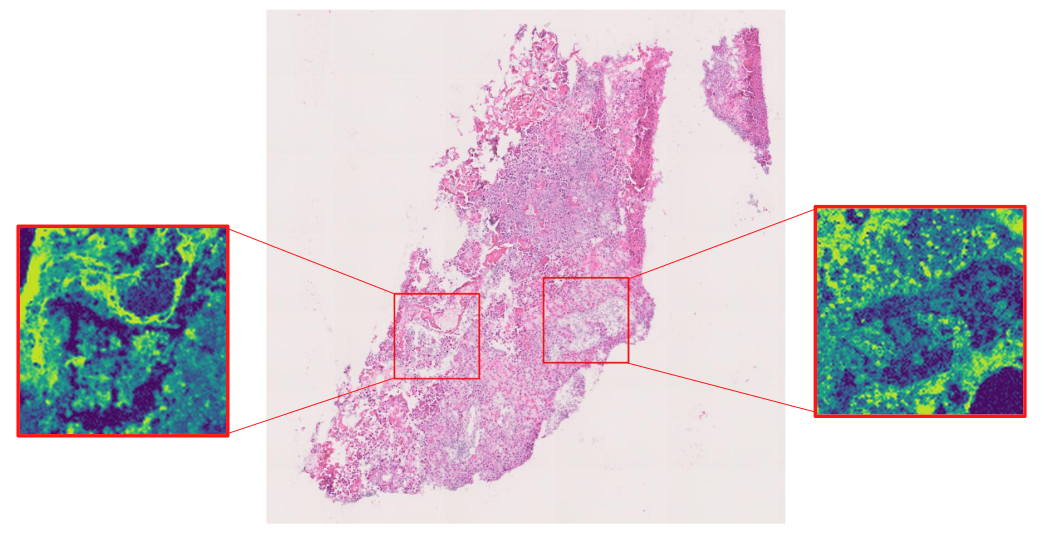
\includegraphics[width=0.8\linewidth]{Images/images_ch_4/stained_sample.png}
    \caption{\textit{Sample} treated with H\&E staining. Two \textit{maps} are magnified and displayed as heatmaps based on Raman data.}
    \label{fig:placeholder}
\end{figure}


\section{Labels}
\label{sec:labels}

Each pixel (spectrum) has been assigned a label, corresponding to a specific type of biological tissue, by a histopathologist.
The classification pipeline started with the preparation of the samples as $12~\mu\mathrm{m}$ slices of tumoral tissue.
Raman spectroscopy was first performed on each slice. The slices were then treated through H\&E staining to allow the histopathologist to assign the labels. Finally, the annotations from the H\&E were directly transferred into the Raman Map.

This process includes two critical points:

\begin{itemize}
    \item Human annotation is region-based rather than pixel-exact, unlike automated classification; errors are therefore particularly common at boundaries between tissues.
    \item Human misclassification of entire areas.
\end{itemize}

However, the provided labels have been considered correct, as is accepted in the state of the art of these studies.


Biological tissues were divided into 13 classes, the most represented of which was the \textit{tumor} class (46,71\%). Occurrences for each class are shown in \Cref{fig:label_distribution} and detailed in \Cref{tab:label-distribution}.


\begin{table}[ht]
    \centering
    \begin{tabular}{|c|l|r|r|}
        \hline
        \textbf{Label} & \textbf{Tissue class} & \textbf{Spectra} & \textbf{\%} \\
        \hline
        2  & Tumor                         & 524\,671 & 46,71 \\
        6  & Tumor stroma                  & 216\,117 & 19,24 \\
        4  & Stroma with inflammation      & 149\,319 & 13,29 \\
        5  & Connective tissue             & 68\,619  & 6,11  \\
        20 & Tumor with necrosis           & 54\,911  & 4,89  \\
        $-1$ & Unlabeled/transparent       & 45\,940  & 4,09  \\
        15 & Artifact                      & 18\,215  & 1,62  \\
        19 & Epithelium (squamous, normal) & 15\,189  & 1,35  \\
        3  & Skeletal muscle cells         & 11\,143  & 0,99  \\
        0  & Necrosis                      & 10\,795  & 0,96  \\
        8  & Glandular tissue              & 4\,203   & 0,37  \\
        10 & Blood vessel                  & 3\,412   & 0,30  \\
        23 & Lymphatic tissue              & 666      & 0,06  \\
        \hline
        \multicolumn{2}{|r|}{\textbf{Total}} & \textbf{1\,123\,200} & \textbf{100} \\
        \hline
    \end{tabular}
    \caption{Per-class composition of the dataset, ordered by abundance. The \textit{unlabeled/transparent} and \textit{artifact} classes are non-tissue classes that are excluded before further analysis.}
    \label{tab:label-distribution}
\end{table}

Among the classes, two do not correspond to any biological tissue and were removed before further analysis: the \textit{unlabeled/transparent} pixels correspond to holes in the tissue (detection of the glass substrate); the \textit{artifacts} from the H\&E staining. Their average spectra also differ from the tissue classes, mainly in the fingerprint region (\Cref{fig:spectra_comparison_discarded}). Keeping them would bias the model towards features unrelated to the tumoral/healthy distinction, so they were excluded from the dataset.

\begin{figure}[H]
    \centering
    \subfloat[Occurrences for each label in the dataset.\label{fig:label_distribution}]{
        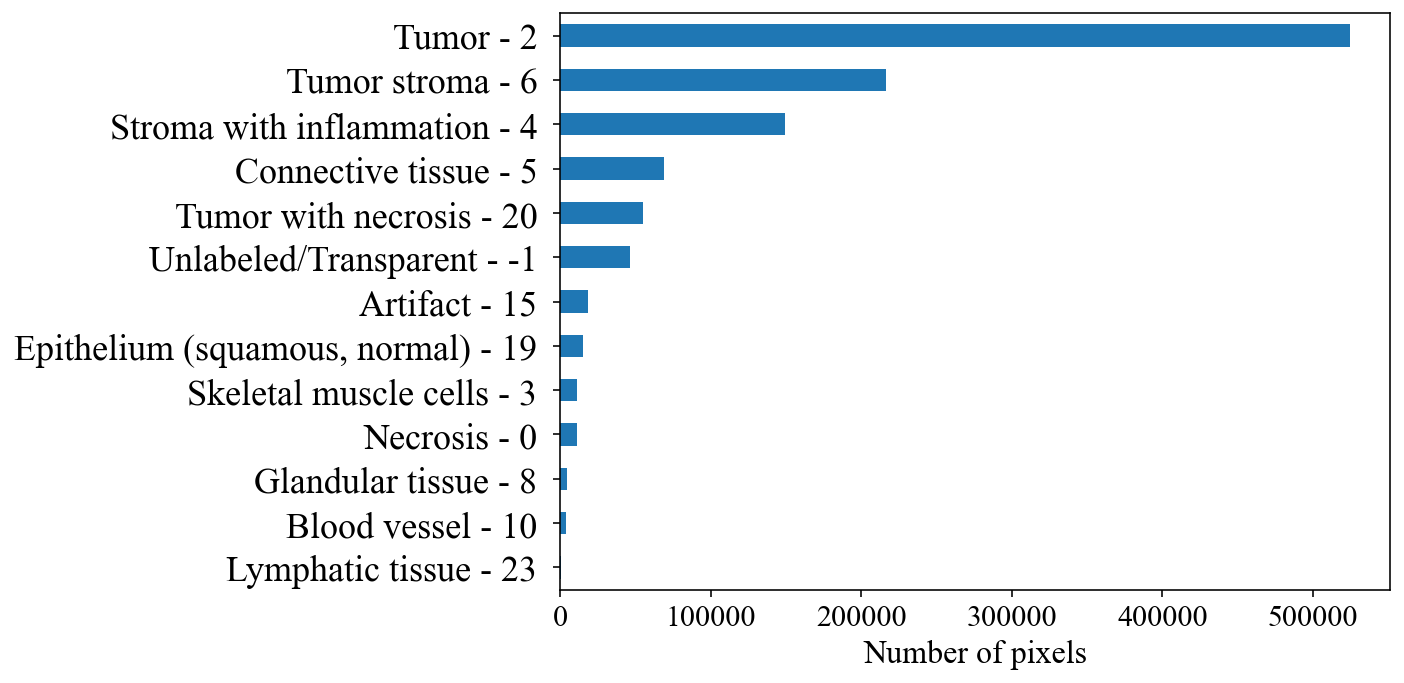
\includegraphics[width=0.45\textwidth]{Images/images_ch_4/label_distributions.png}
    }
    \hfill
    \subfloat[Binary grouping by tumoral and healthy spectra after discarding unlabeled, transparent pixels and artifacts.\label{fig:binary_label_distribution}]{
        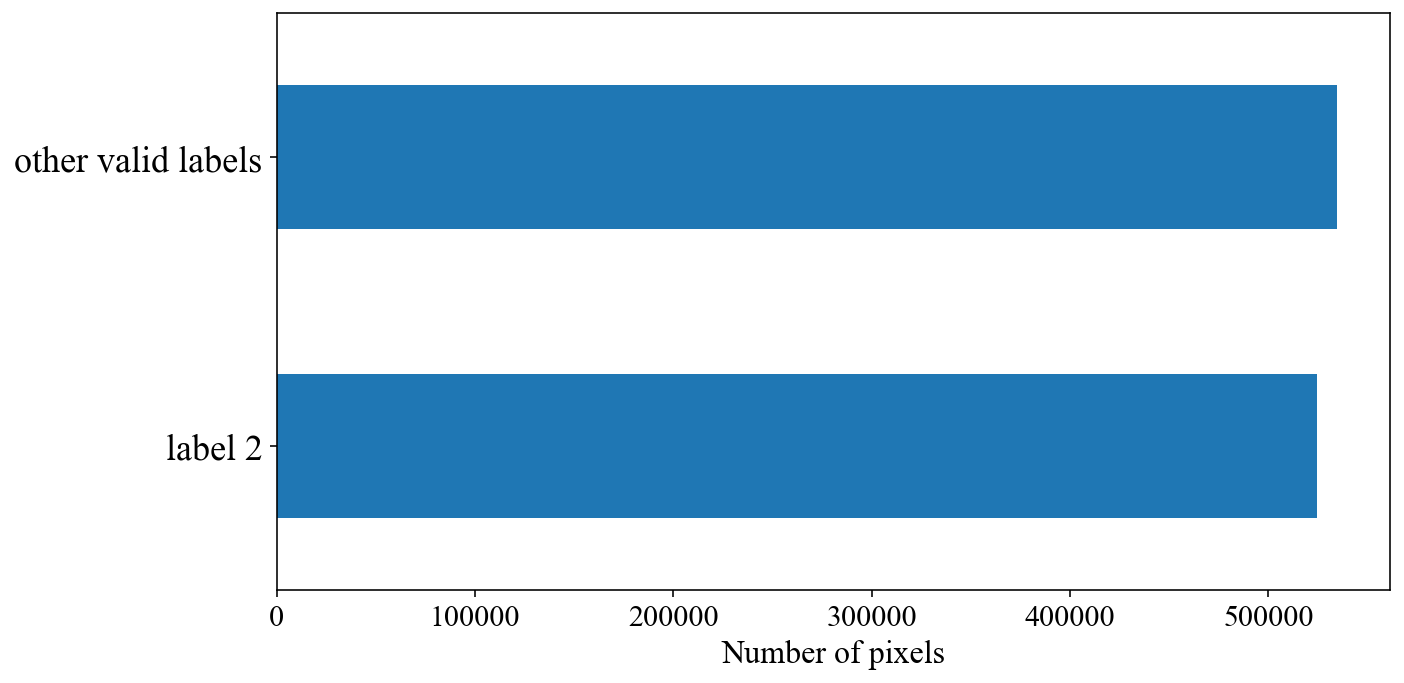
\includegraphics[width=0.45\textwidth]{Images/images_ch_4/binary_label_distribution.png}
    }
    \caption{Distribution of labels in the dataset.}
    \label{fig:label_distributions}
\end{figure}


\section{Spectra}
\label{sec:spectra}
For the cross-class comparisons reported below, the averaged spectra were further normalized with the standard normal variate (SNV) transform, which centers each spectrum and scales it to unit standard deviation, so that band shapes can be compared independently of overall intensity.

In a preliminary visual analysis, the average spectrum for each class has been computed. At the major Raman peaks the standard deviation across individual spectra corresponds to 12–20\% of the peak height. Relative to the local signal intensity, this dispersion is small near the peaks, although it grows noticeably in the weak baseline regions (bands 30--200), where the standard deviation becomes roughly 30\% of the local mean.

\begin{figure}[ht]
    \centering
    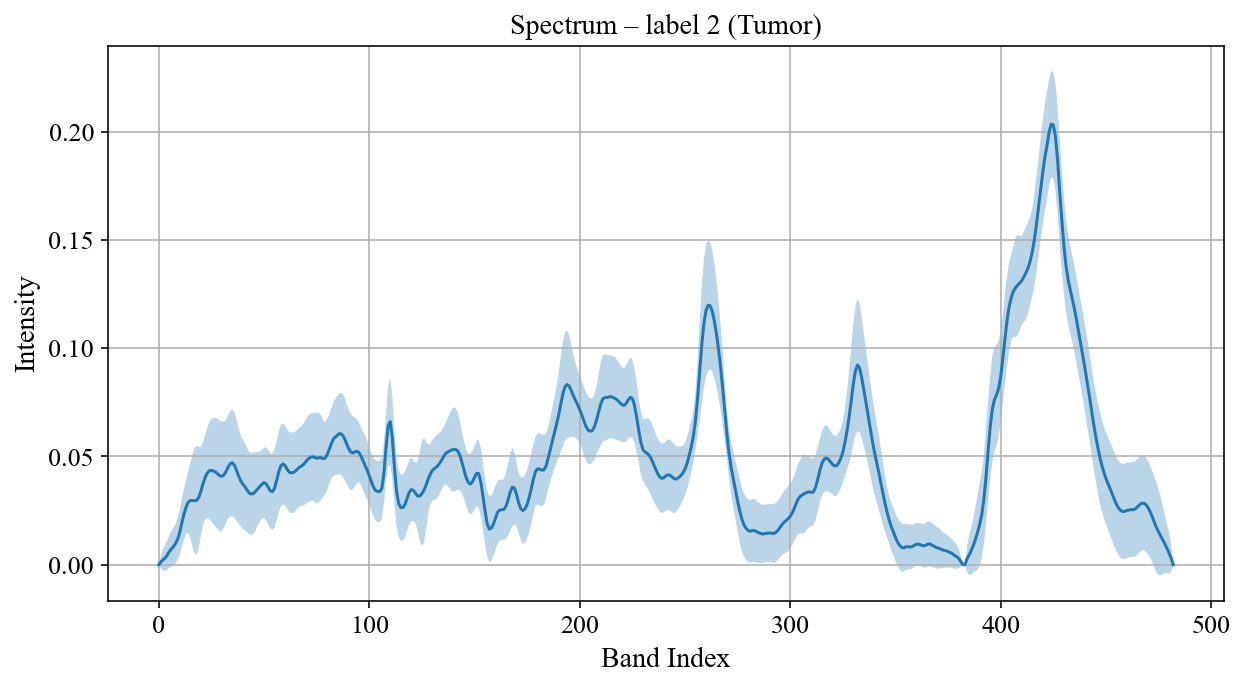
\includegraphics[width=0.65\linewidth]{Images/images_ch_4/spectrum_avg_tumor.png}
    \caption{Average spectrum for the \textit{tumor} label. The shaded band shows $\pm1$ standard deviation across spectra. The \textit{fingerprint region} and \textit{CH region} are joined at band n.390, where the intensity is 0.}
    \label{fig:spectrum_avg_tumor}
\end{figure}

All classes appear to have the same trends, with multiple similar peaks in the \textit{fingerprint region} (bands 0--382, or equivalently 500--1800 $\mathrm{cm}^{-1}$) and a major peak in the \textit{CH region} (bands 383--483, or equivalently 2800--3000 $\mathrm{cm}^{-1}$). The only exceptions are represented by \textit{unlabeled/transparent}, \textit{artifact} and \textit{necrosis} pixels, which differ from the others mainly in the fingerprint region (\Cref{fig:spectra_comparison_discarded}).


\begin{figure}[H]
    \centering
    \subfloat[\textit{tumor} spectrum against the excluded non-tissue classes (\textit{unlabeled/transparent}, \textit{artifact}) and \textit{necrosis}.\label{fig:spectra_comparison_discarded}]{
        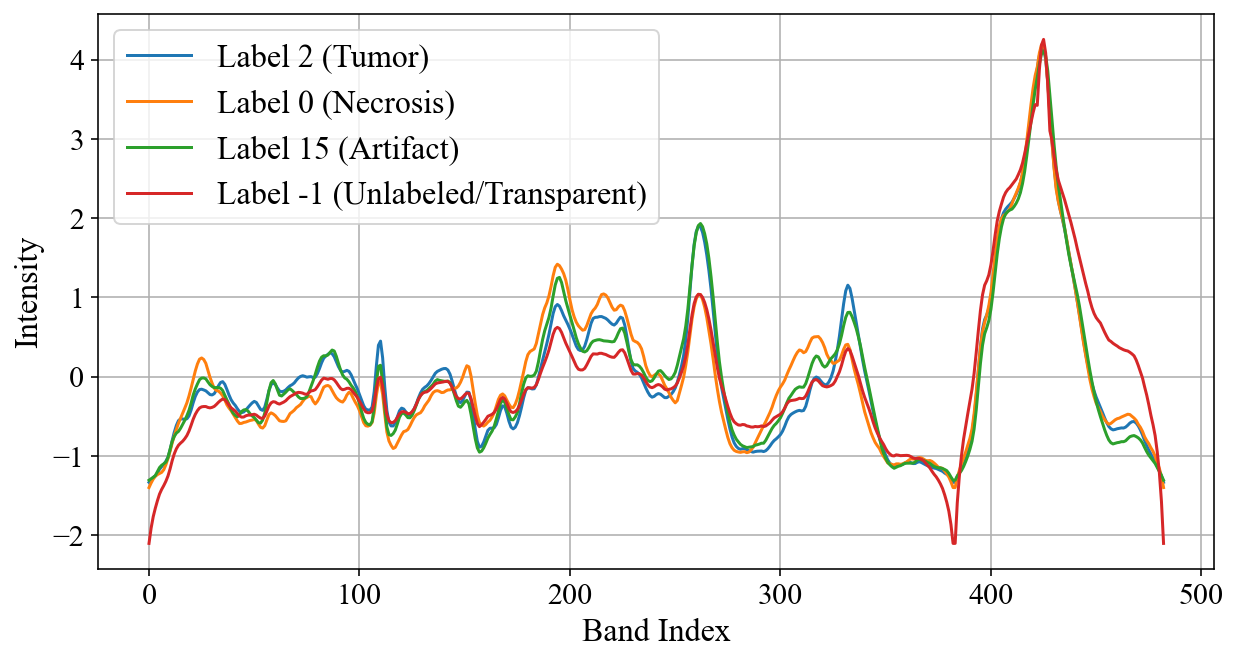
\includegraphics[width=0.45\textwidth]{Images/images_ch_4/spectra_comparison_discarded.png}
    }
    \hfill
    \subfloat[\textit{tumor} spectrum against the most represented healthy classes.\label{fig:spectra_comparison_similar}]{
        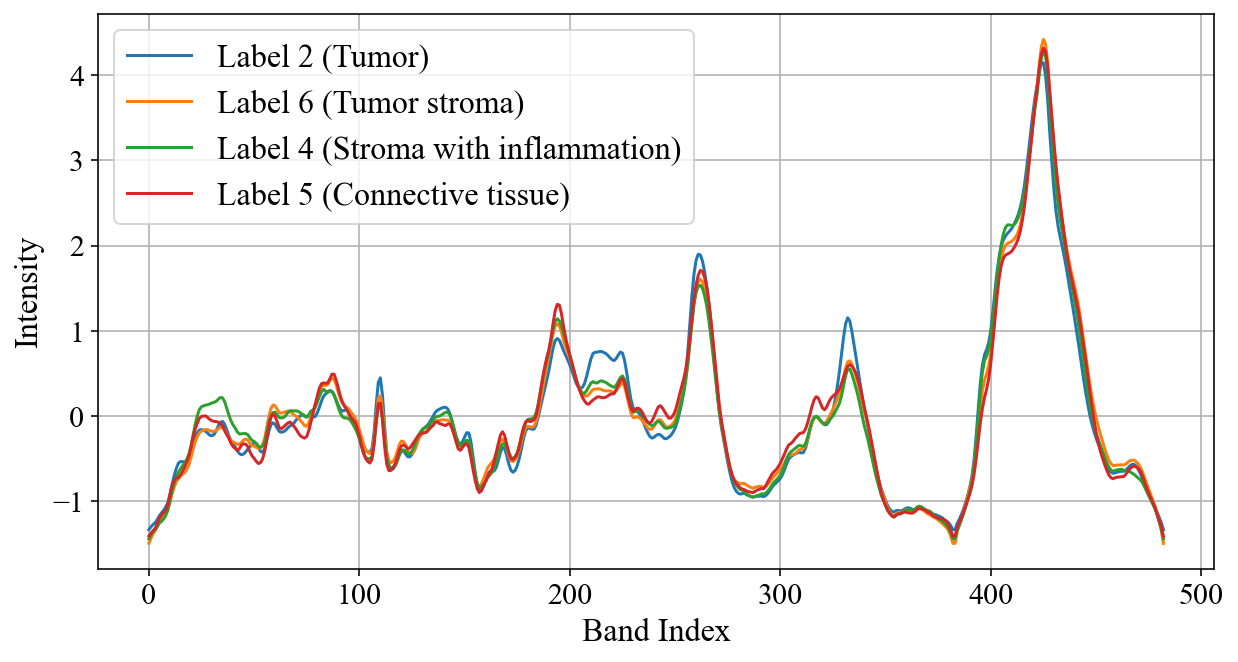
\includegraphics[width=0.45\textwidth]{Images/images_ch_4/spectra_comparison_similar.png}
    }
    \caption{Comparison of spectra for different classes. The spectra are averaged across each label and SNV-normalized.}
    \label{fig:spectra_comparisons}
\end{figure}


\section{Definition of the binary classification problems}
\label{sec:binary_classification}

In the prospect of training a binary classification ANN it was necessary to set a choice for the binary labeling to be used as ground truth for training and performance verification.


Two strategies were considered for this task:
\begin{itemize}
    \item \textbf{\textit{Tumor} vs. \textit{healthy} discrimination}
    \\Grouping all or part of the labels under the \textit{Tumor} and \textit{Healthy} macro-classes.
    \item \textbf{Single class discrimination}
    \\Choosing a class of particular interest other than \textit{Tumor} and discarding all others
\end{itemize}


The choice had to account for the following criteria:
\begin{itemize}
    \item \textbf{Biological relevance:} the distinction needs to have useful applications.
    \item \textbf{Numerosity:} the two groups had to be comparable in size for the ANN to train and perform inference correctly.
    \item \textbf{Discernability:} the average spectral differences between classes change classification performance and usefulness.
\end{itemize}

The first approach is the one with the most clinical relevance. Successful classification of tumoral areas against general healthy tissue would be the most versatile result possible, with further single-class distinction to be performed later depending on need. The balance between the two classes would also be close to 50/50, allowing to use the whole dataset for training and testing of the ANN. This approach presents however multiple critical points.
The \textit{healthy} macro-class, including numerous tissue types, is very heterogeneous (high intra-class variance), leading to poor feature individuation or bias towards the major class.
The \textit{tumor} macro-class, which always includes the \textit{tumor (2)} label, could also comprise the \textit{tumor with necrosis (20)} and the \textit{necrosis (0)} labels, since necrotic tissue is expected to be adjacent to tumors; necrotic tissue, however, shows high variance (\Cref{fig:spectra_comparison_discarded}) due to structural degradation of the cells, leading to problems similar to the ones of the \textit{healthy} macro-class.


The second approach, using isolated classes, will reduce intra-class variance and allow the model to learn the class-specific patterns, thus improving performance.
Due to the class imbalance (tumor alone being 46,71\% of the dataset), the classes will not be equal in numerosity anymore, requiring rebalancing by discarding part of the available training data. The model is then trained on a reduced number of spectra. Due to the size of the dataset ($>$1\,000\,000 spectra) and the strong spatial correlation between adjacent pixels, which makes neighbouring spectra highly redundant, the data can be substantially subsampled with little loss of information, provided that spectra from every sample are retained. This reduces the possible choices for \textit{healthy} labels to the most numerous ones, i.e.\ \textit{tumor stroma (6)}, \textit{stroma with inflammation (4)} and \textit{connective tissue (5)} (\Cref{fig:label_distribution}).

Regarding discernability, the most similar tissues are also the most clinically confusable. Being able to discriminate would then be the most valuable result. The three possible healthy classes show a comparable degree of similarity to the tumor (\Cref{fig:spectra_comparison_similar}); each therefore constitutes an equally valid choice, with no class being a priori better suited than the rest from a separability standpoint.

Clinically, each label can be relevant in different ways:
\begin{itemize}
    \item \textbf{Tumor stroma:} is the supportive environment for future tumoral growth (though still healthy). It sits right at the boundary between tumoral tissue and healthy tissue, thus it is of primary interest for surgical margin assessment.
    \item \textbf{Stroma with inflammation:} Stroma infiltrated by immune cells. Related to \textit{tumor stroma}, they often overlap and are classified based on the histopathologist's judgement and not due to strict biological distinction. Stroma with inflammation can be also unrelated to tumoral activity, although the scale of the problem (few $\mu\mathrm{m}$) makes this possibility very unlikely.
    \item \textbf{Connective tissue:} Unaltered collagen rich tissue. Would serve to the same purpose of the macro-class distinction proposed previously.
\end{itemize}

Two binary problems are therefore taken forward to the classification stage. The first, \textit{tumor} vs.\ \textit{healthy}, groups all valid non-tumor classes into a single \textit{healthy} macro-class: it targets the broad, clinically versatile question and keeps the two groups close to 50/50, allowing the whole dataset to be used. The second, \textit{tumor} vs.\ \textit{tumor stroma}, is a single, surgically motivated pairing for margin assessment; building the \textit{healthy} side from the most numerous single class yields a spectrally homogeneous and balanced training set, for which better performance is expected.


\begin{figure}[H]
    \centering
    \subfloat[\textit{Tumor} vs.\textit{healthy} classification.\label{fig:heatmap-tumor-vs-healthy}]{
        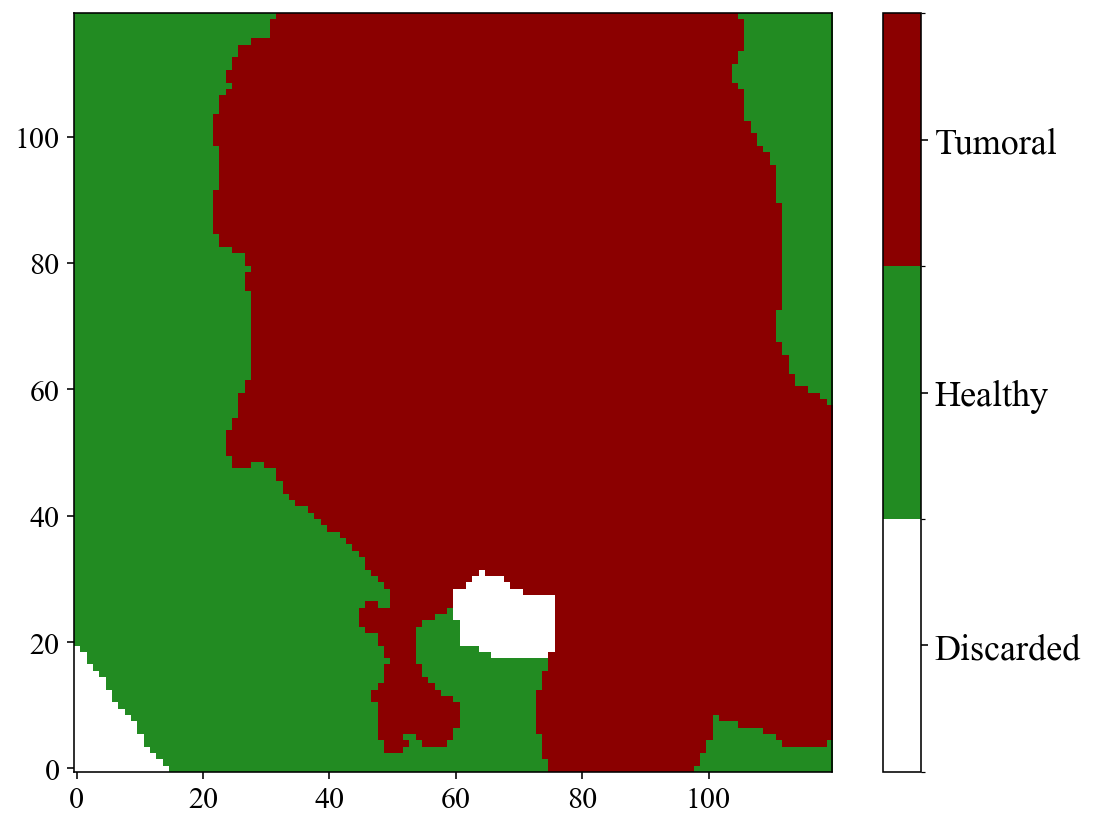
\includegraphics[width=0.45\textwidth]{Images/images_ch_4/heatmap_tumor_vs_healthy.png}
    }
    \hfill
    \subfloat[\textit{Tumor} vs.\textit{tumor stroma} classification.\label{fig:heatmap-tumor-vs-stroma}]{
        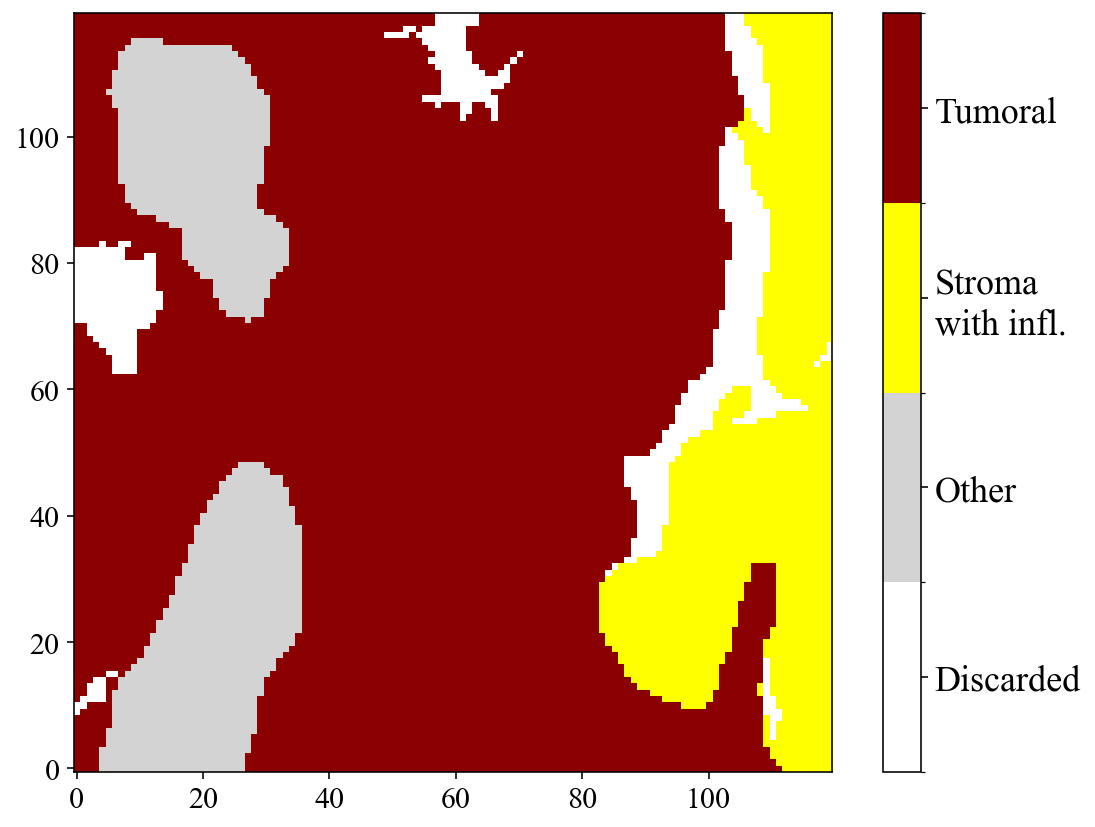
\includegraphics[width=0.45\textwidth]{Images/images_ch_4/heatmap_tumor_vs_stroma.png}
    }
    \caption{Maps with highlighted labels based on classification approach. As is often the case, \textit{tumor stroma} is located at the boundary of the \textit{tumoral} region.}
    \label{fig:heatmap_classification}
\end{figure}



\section{Network architectures}
\label{sec:architectures}

The classification stage was based on three model architectures (S, M, L) that varied in width (\cref{tab:architectures}). A grid search was performed by varying model size and multiple hyperparameters to determine the best possible combination. A model that is too small would be expected to underfit, not learning enough relevant patterns to categorize well enough, whereas an overly large one would overfit, memorizing the dataset rather than generalizing.

\begin{table}[ht]
    \centering
    \small
    \begin{tabular}{|l|c|c|c|c|}
        \hline
        \textbf{Model} & \textbf{Hidden layers} & \textbf{Neurons/layer} & \textbf{Output} \\
        \hline
        Small (S)  & 2 & 16, 8 & 1 (sigmoid) \\
        Medium (M) & 2 & 64, 32 & 1 (sigmoid) \\
        Large (L)  & 3 & 128, 64, 16 & 1 (sigmoid) \\
        \hline
    \end{tabular}
    \caption{Architecture of the three model sizes (S, M, L). All hidden layers use ReLU activation (\cref{subsec:activation_functions}); the output layer is a single sigmoid unit for binary classification (\cref{subsec:bce}).}
    \label{tab:architectures}
\end{table}

The models all consisted of \textit{dense} (fully connected) layers.

All the hidden layers used ReLU as activation functions and the number of input units is set to the number of retained PC components (itself a hyperparameter, selected jointly with the architecture, see \cref{sec:training}), while the output neurons had a sigmoid activation.


\section{Data splitting and cross validation}
\label{sec:data_splitting}

The spectra in the dataset are spatially correlated: neighboring pixels show similar patterns and peaks. Therefore, a simple random split of the whole dataset into training, validation and test sets would result in spectra from the same map or sample being present in multiple divisions. Such a split would let the model memorize sample-specific signatures and give misleading results due to data leakage.

Furthermore, because different maps and samples contain different mixes of biological tissue, the performance of the model in testing and validation is heavily dependent on which samples happen to fall in each set.

A splitting protocol based on Sample IDs was implemented to solve both problems at once, combining a Sample-ID-based split with cross validation into a single pipeline:
\begin{enumerate}
    \item The dataset is divided by Sample ID into $k$ \textit{stratified} folds, where the stratification means keeping the ratio of the two labels close to 1:1 in each fold (by downsampling the majority class) while ensuring that no Sample ID is split across folds.
    \item At each of the $k$ iterations, one fold is held out as the \textit{test} set, while the remaining $k-1$ folds form the training pool.
    \item An internal \textit{validation} set is carved out of the training pool (again split by Sample ID, to avoid leakage), leaving the rest as the actual training set. The validation set is used to monitor the model during training (e.g. for early stopping), while the test fold is reserved for final evaluation only.
\end{enumerate}

Throughout this splitting protocol, $k$ denotes the number of cross-validation folds.

This is repeated for all $k$ folds, so that every sample is used exactly once for testing. Results are saved for each fold and then averaged, to balance out 'easy' and 'difficult' folds and obtain a representative estimate of performance rather than one dependent on a single, possibly lucky, split.

If PCA was performed on the whole dataset, the test set would be decomposed in PCs that were fitted on the training set and vice-versa. This would once again lead to data leakage. To avoid this issue, the split was performed on the raw dataset, then PCA was refitted on each training set ($k$ PCAs performed each time, once per split).

For this dataset, cross validation was performed with $k=5$ folds, maintaining roughly 5 sample IDs per fold ($\sim20\%$ of the dataset).


\section{Training protocol and hyperparameter search}
\label{sec:training}

There are multiple hyperparameters that are not fixed a priori, for which an optimal value has to be found to make the model perform best. Those parameters comprise: network size, number of retained PCs and batch size.
To choose between them, a grid search was performed. For each hyperparameter, a list of possible values was chosen, then the model was trained and tested for every possible combination of those values (said combinations are called the \textit{search space}).

Network size and number of retained PCs were searched jointly first, over the three possible network sizes S, M, L (\cref{sec:architectures}) and thirteen values for the number of retained principal components $N_{PC} \in \{1, 2, 3, 5, 10, 20, 30, 50, 100, 200, 300, 400, 483\}$, where the last value corresponds to full dimensionality (equivalent to training on the full Raman spectra).
The full search, using 5-fold cross validation (\cref{sec:data_splitting}), meant training $3\times 13\times 5 = 195$ models and comparing the $3\times 13 = 39$ results.

To reduce computational complexity, once the best architecture and $N_{PC}$ combination was selected, batch size was tuned separately on this fixed configuration, over six values of the batch size $N_\mathcal{B} \in \{512, 1024, 2048, 4096, 8192, 16384\}$. Batch sizes were chosen as powers of 2 due to convention and minor optimization in computer memory.

As explained in \cref{subsec:pca_svd}, PCA is fitted on the full dimensional spectrum, then the required number of PCs are selected by keeping only the first columns of the projected data matrix. This avoids the computational burden of reducing dimensionality for every training instance.

Two callbacks were implemented to control training:

\begin{itemize}
    \item \textit{Early stopping:} training stops when the validation AUC (Area Under the Curve, explained in \cref{sec:evaluation_metrics}) doesn't improve for 10 consecutive epochs, restoring the weights to the best epoch.
    \item \textit{Learning rate reduction on plateau:} when validation loss fails to improve for 4 consecutive epochs, the learning rate $\eta$ is reduced by half, down to a minimum of $\eta = 10^{-6}$. This allows for finer tuning compared to the relatively coarse \textit{Adam} steps.
\end{itemize}

All stochastic parts of the pipeline (i.e.\ fold assignment, the split within each fold, and majority-class downsampling) use a fixed random seed, so that results are deterministic and comparable across the grid, although the model's weight initialization done by Keras is not fixed. Differences in metrics between configurations reflect the architecture/$N_{PC}$ choice itself, not casual variation from a different random split. The variations caused by the different initializations are negligible ($\sim1\%$ on AUC) compared to those given by the split.



\section{Spatial post-processing}
\label{sec:spatial_post_processing}

The network classifies each pixel in isolation, learning to recognise its composition solely from the corresponding spectrum and not accounting for spatial structure. However, since the spectra are acquired within maps, they are also associated with spatial coordinates \((x,y)\) and consequently adjacent pixels are correlated, as they often belong to the same biological region.

To introduce the spatial classification problem and test if these correlations are actually relevant in order to improve predictions, a spatial filter is used. Starting from the probabilities predicted by the model for each pixel, this filter computes the average on a spatially arbitrary window, correcting it on the basis of the context of the predicted neighbouring probabilities.
This step does not alter the neural network's intrinsic capacity, since spatial information never enters the network's training phase and is applied only after inference.

Let \(p(x,y)\) be the probability predicted by the model for the positive class at the pixel located at coordinates \((x,y)\). Using a \(w \times w\) average filter, the smoothed probability \(\tilde{p}(x,y)\) can be written as

\begin{equation}
    \tilde{p}(x,y) =
    \frac{1}{w^2}
    \sum_{(i,j)\in(x,y)} p(i,j)
    \label{eq:spatial_smoothing}
\end{equation}

The kernel size $w$ (not to be confused with the number of cross-validation folds $k$, \cref{sec:data_splitting}) is a configurable parameter and different sizes were tested such as \(3 \times 3\), \(5 \times 5\), \(7 \times 7\), \(10 \times 10\), \(15 \times 15\).

After smoothing, the probabilities are converted into binary labels based on the \textit{decision threshold} $\tau$ (its role in the precision/recall tradeoff is discussed in \cref{sec:evaluation_metrics}):
\begin{equation}
    \hat{y}(x,y) =
    \begin{cases}
        1, & \tilde{p}(x,y) > \tau,\\
        0, & \tilde{p}(x,y) \leq \tau,
    \end{cases}
    \label{eq:threshold_after_smoothing}
\end{equation}

The result to be obtained is a reduction in isolated and inconsistent predictions due to the instability of the classifier or noise in favor of greater spatial coherence. Among the limitations of this implementation is definitely the risk of propagating incorrect local predictions if an area that has produced incorrect probabilities is large enough to influence neighboring pixels. Overall, raw and smoothed predictions must be compared based on global metrics and prediction maps.

\section{Evaluation metrics}
\label{sec:evaluation_metrics}

Accuracy is often not the best metric to consider in order to evaluate the performance of a model. When the dataset is not balanced, accuracy could be very high although the model does not perform well. For example, if the dataset was composed at 90\% by tumoral cells, even a model that just classifies as 'tumoral' every pixel would achieve 90\% accuracy, although not predicting anything at all.

A better way to evaluate a model is through the \textit{confusion matrix}, which shows how many times instances of class A are classified as B, for every possible combination of classes. Each row in a confusion matrix represents an \textit{actual class}, while each column represents a \textit{predicted class}.
For a binary classifier, the \textit{true positive} TP and \textit{true negative} TN lie on the main diagonal, while the off-diagonal terms represent \textit{false positives} FP and \textit{false negatives} FN (\cref{fig:confusion_matrix}).
Since the absolute counts (TP, FP, TN, FN) can be very big numbers when dealing with large datasets, another way to represent the confusion matrix is through the classification rates (\cref{fig:confusion_matrix_rates}), defined hereafter.

The \textit{true positive rate} (TPR), also called \textit{recall}, is the ratio of positive instances that are correctly detected by the classifier:

\begin{equation}
    \text{TPR (\textit{recall})} = \frac{\text{TP}}{\text{TP}+\text{FN}}
\end{equation}


The \textit{false negative rate} (FNR) is the ratio of positive instances that are incorrectly detected by the classifier (the denominator is the same as for the TPR):

\begin{equation}
    \text{FNR} = \frac{\text{FN}}{\text{TP}+\text{FN}}
\end{equation}

The \textit{true negative rate} (TNR), also called \textit{specificity}, and \textit{false positive rate} (FPR) follow the same logic, applied to the negative class:

\begin{equation}
    \text{TNR (\textit{specificity})} = \frac{\text{TN}}{\text{TN}+\text{FP}}
\end{equation}

\begin{equation}
    \text{FPR} = \frac{\text{FP}}{\text{TN}+\text{FP}}
\end{equation}

\begin{figure}[ht]
    \centering
    \subfloat[Confusion matrix expressed as absolute counts.\label{fig:confusion_matrix}]{
        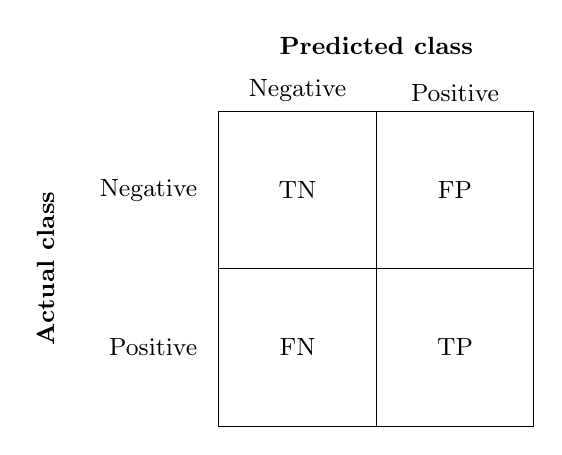
\begin{tikzpicture}[font=\small]
            \draw (0,0) rectangle (2,2);
            \draw (2,0) rectangle (4,2);
            \draw (0,-2) rectangle (2,0);
            \draw (2,-2) rectangle (4,0);
            \node at (1,1) {TN};
            \node at (3,1) {FP};
            \node at (1,-1) {FN};
            \node at (3,-1) {TP};
            \node[above] at (1,2) {Negative};
            \node[above] at (3,2) {Positive};
            \node[anchor=east] at (-0.15,1) {Negative};
            \node[anchor=east] at (-0.15,-1) {Positive};
            \node[above] at (2,2.6) {\textbf{Predicted class}};
            \node[rotate=90] at (-2.2,0) {\textbf{Actual class}};
        \end{tikzpicture}
    }
    \hfill
    \subfloat[Confusion matrix expressed as classification rates.\label{fig:confusion_matrix_rates}]{
        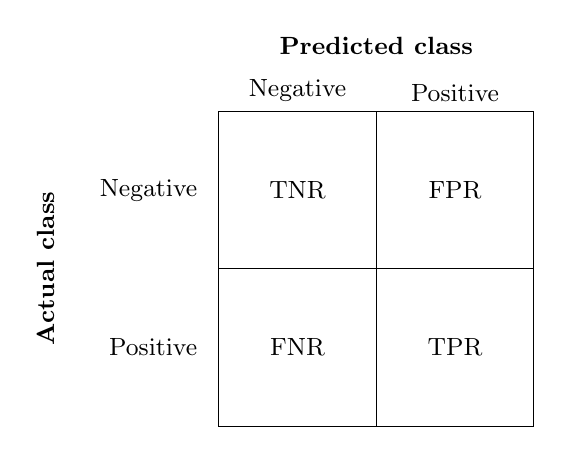
\begin{tikzpicture}[font=\small]
            \draw (0,0) rectangle (2,2);
            \draw (2,0) rectangle (4,2);
            \draw (0,-2) rectangle (2,0);
            \draw (2,-2) rectangle (4,0);
            \node at (1,1) {TNR};
            \node at (3,1) {FPR};
            \node at (1,-1) {FNR};
            \node at (3,-1) {TPR};
            \node[above] at (1,2) {Negative};
            \node[above] at (3,2) {Positive};
            \node[anchor=east] at (-0.15,1) {Negative};
            \node[anchor=east] at (-0.15,-1) {Positive};
            \node[above] at (2,2.6) {\textbf{Predicted class}};
            \node[rotate=90] at (-2.2,0) {\textbf{Actual class}};
        \end{tikzpicture}
    }
    \caption{Confusion matrix for a binary classifier, expressed as absolute counts (a) and as classification rates (b).}
\end{figure}

Another useful metric is \textit{precision}, which indicates the accuracy of the positive predictions, expressed as:

\begin{equation}
    \textit{precision} = \frac{\text{TP}}{\text{TP}+\text{FP}}
\end{equation}

Increasing precision reduces recall, and vice versa. This is called the \textit{precision/recall tradeoff}. The ratio between the two is determined through a \textit{decision threshold}. For each instance, the model computes a score based on the decision function, and if that score is greater than the threshold, it assigns the instance to the positive class, or else it assigns it to the negative class.

It is also useful to combine precision and recall into a single metric called the $F_1$ score, in particular when a simple way to compare two classifiers is needed. The $F_1$ score is the harmonic mean of precision and recall, which gives more weight to low values compared to a regular mean

\begin{equation}
    F_1 = \frac{2}{\dfrac{1}{\text{precision}} + \dfrac{1}{\text{recall}}} = 2 \times \frac{\text{precision} \times \text{recall}}{\text{precision} + \text{recall}}
\end{equation}

however, the $F_1$ score favors classifiers that have similar precision and recall, which might not be optimal for every classifier. In some cases precision might be more important than recall, while in other the opposite might be true.

In this work, recall is undoubtedly more important. Classifying a healthy pixel as tumoral has fewer consequences than failing to catch a tumoral one through low recall.

The \textit{receiver operating characteristic} (ROC) curve is another common tool used with binary classifiers. It plots TPR (\textit{recall}) against FPR. The tradeoff is always present: the higher the recall, the more false positives (FPR) the classifier produces. The dashed line in \cref{fig:roc_curve} represents the ROC curve of a purely random classifier; a good classifier stays as far away from that line as possible (toward the top-left corner). One way to compare classifiers is to measure the area under the curve (AUC). A perfect classifier will have a ROC AUC equal to 1, whereas a purely random classifier will have a ROC AUC equal to 0.5.

\begin{figure}[H]
    \centering
    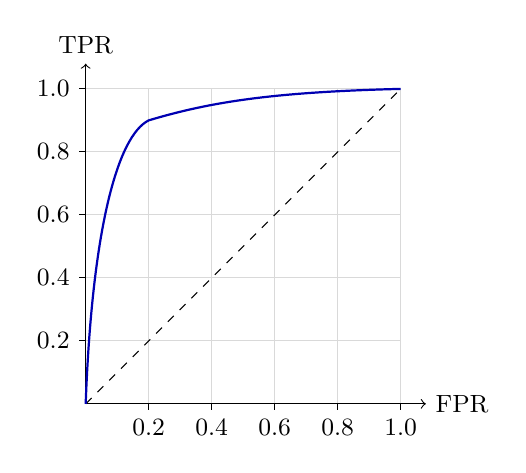
\begin{tikzpicture}[font=\small, x=4cm, y=4cm]
        \draw[gray!30] (0,0) grid[step=0.2] (1,1);
        \draw[->] (0,0) -- (1.08,0) node[right] {FPR};
        \draw[->] (0,0) -- (0,1.08) node[above] {TPR};
        \foreach \t in {0.2,0.4,0.6,0.8,1.0} {
            \draw (\t,0) -- (\t,-0.02) node[below] {\t};
            \draw (0,\t) -- (-0.02,\t) node[left] {\t};
        }
        \draw[dashed] (0,0) -- (1,1);
        \draw[blue!70!black, thick] (0,0) .. controls (0.02,0.55) and (0.1,0.85) .. (0.2,0.9)
            .. controls (0.4,0.96) and (0.6,0.99) .. (1,1);
    \end{tikzpicture}
    \caption{General shape of a ROC curve (solid) compared to a random classifier (dashed diagonal).}
    \label{fig:roc_curve}
\end{figure}


\section{Software and computational tools}
\label{sec:software_tools}

The code for this work was written in Python (version 3.11) and made use of multiple libraries for the dataset's exploration, implementation of PCA, Neural networks and plotting.

The dataset was stored in a \texttt{.parquet} file, a column-based format designed for efficient data storage and retrieval and widely used in clinical data analytics, medical research, and machine learning. The information from the dataset was retrieved through \texttt{PyArrow}, an engine optimized for managing large datasets (in this case more than one million rows). Once the dataset was loaded into a data frame, manipulations such as filtering and label mapping were performed with \texttt{Pandas}, while numerical array operations relied on \texttt{NumPy}.

Dimensionality reduction and PCA were implemented by importing Scikit-Learn's PCA class as \texttt{sklearn.decomposition.PCA}. This import made available ad hoc functions and variables such as \texttt{.fit\_transform()} and \texttt{.explained\_variance\_ratio\_}, then used for computing SVD and the plotted data.

The dataset was divided into folds and split into training, validation and test sets using \texttt{GroupShuffleSplit} and \texttt{StratifiedGroupKFold} from Scikit-Learn's \texttt{model\_selection} module.

The ANN architectures were built through TensorFlow's Keras API as \texttt{Sequential} models of \texttt{Dense} layers. As described in \cref{sec:training}, training was controlled by two callbacks: \texttt{EarlyStopping} and \texttt{ReduceLROnPlateau}. AUC and loss were tracked during training in order to plot their values for each epoch, while test set performances on the metrics defined in \cref{sec:evaluation_metrics} were computed with Scikit-learn's \texttt{recall\_score}, \texttt{roc\_auc\_score}, \texttt{roc\_curve}, \texttt{confusion\_matrix}, \texttt{precision\_score} and \texttt{f1\_score} functions.
The final spatial smoothing step (\cref{sec:spatial_post_processing}) was implemented with \texttt{scipy.ndimage.generic\_filter}, which allows the smoothing defined in \cref{eq:spatial_smoothing} to be applied directly.

Finally, all the figures related to the dataset were generated with \texttt{Matplotlib} and \texttt{Seaborn} (a library built on top of the former, particularly useful for plotting annotated heatmaps).

All the stochastic steps (fold and validation splitting, class balancing, PCA fitting, and the ANN's weight initialization) were run with a fixed seed in order to guarantee reproducibility.

% LINK TO THE REPO

% The full implementation is available at \url{https://github.com/claudiocaaruso/VibraAI}.